\documentclass[xcolor=pdftex,x11names,table,hyperref]{beamer}

\usepackage{verbatim}
\usepackage{setspace}
\usepackage{url}
\usepackage{xcolor} % See documentation PDF at http://www.ctan.org/pkg/xcolor
\definecolor{darkgreen}{rgb}{0,0.3,0}
\definecolor{darkblue}{rgb}{.05,.05,.30}
\definecolor{lightgrey}{rgb}{0.65,0.65,0.65}
\usepackage{tikzsymbols}
\usetikzlibrary{matrix,arrows,positioning,automata,shadows,shapes.geometric}


\setbeamertemplate{section in toc}[sections numbered]
\setbeamertemplate{subsection in toc}[subsections numbered]
\setbeamertemplate{subsubsection in toc}[subsubsections numbered]
\usetheme{Singapore}
\setbeamertemplate{navigation symbols}{}
\setbeamertemplate{footline}{%
\vspace{0.0em}%
\hspace{0.5em}%
{\color[rgb]{.1,.1,.1} \insertframenumber{}~/~\inserttotalframenumber}
}

\newcommand{\code}[1]{{\color{darkgreen}\texttt{#1}}}
\newcommand{\detail}[1]{{\color{lightgrey}\small{}#1}}
\newcommand{\teeny}[1]{\scalebox{0.09}{#1}}
\newcommand{\tablecolors}{\rowcolors{2}{blue!12}{white}} % Cool table colors


\begin{document}

\title{\LARGE{Words} \\[1.0em] \small{and their abstractions} \\[1.5em]
 %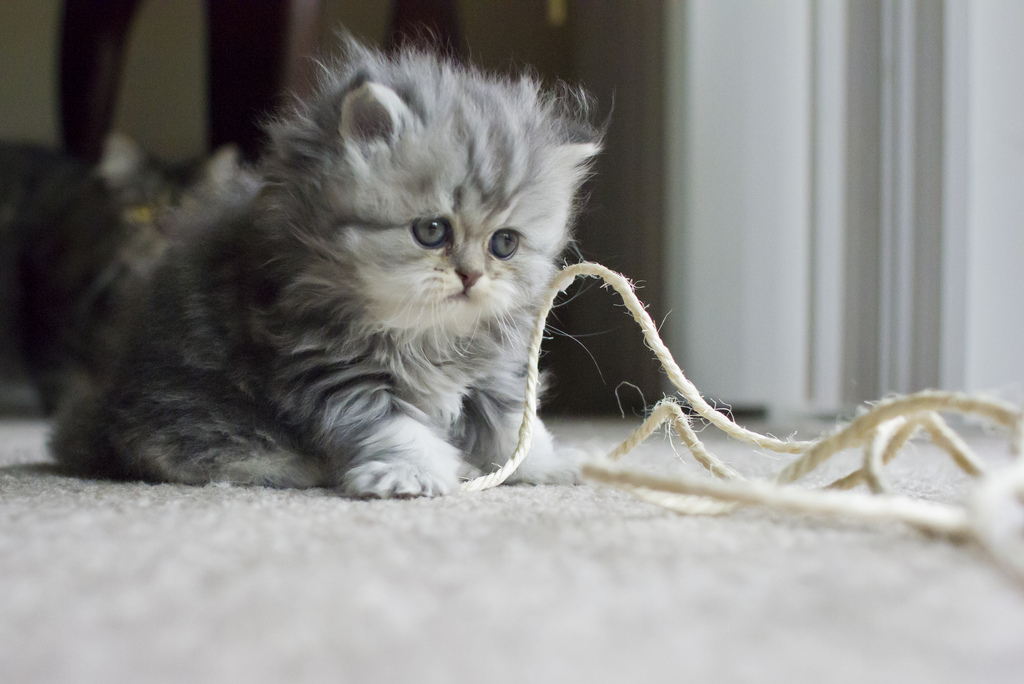
\includegraphics[width=0.5\textwidth]{images/kitten_string_flickr_albaraa.jpg} \\[-1.0em]
 %\small{Possibilities} \\[1.0em]
 %LT1 \\[1.0em]
 }
\author{\href{http://jon.dehdari.org}{Jon Dehdari}}
\frame{\titlepage}

% examples: days of week, company names, first/last names
\begin{frame}{Too Many Words!}
	{\center 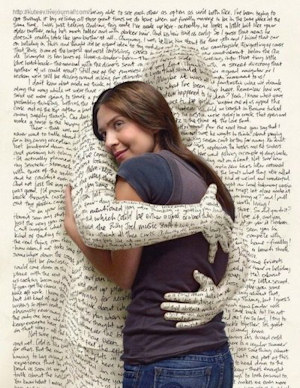
\includegraphics[width=0.33\textheight]{images/word-lover.jpg}}
\begin{itemize}
	\item Languages have too many words for statistical models of language
	\pause
	\item We need some way to generalize them
	\pause
	\item Let's treat some words like other words
\end{itemize}
\end{frame}

\begin{frame}{}
\begin{itemize}
	\item Words can be grouped together into equivalence classes to help reduce data sparsity and better generalize the data.

\begin{center}
	\pause
	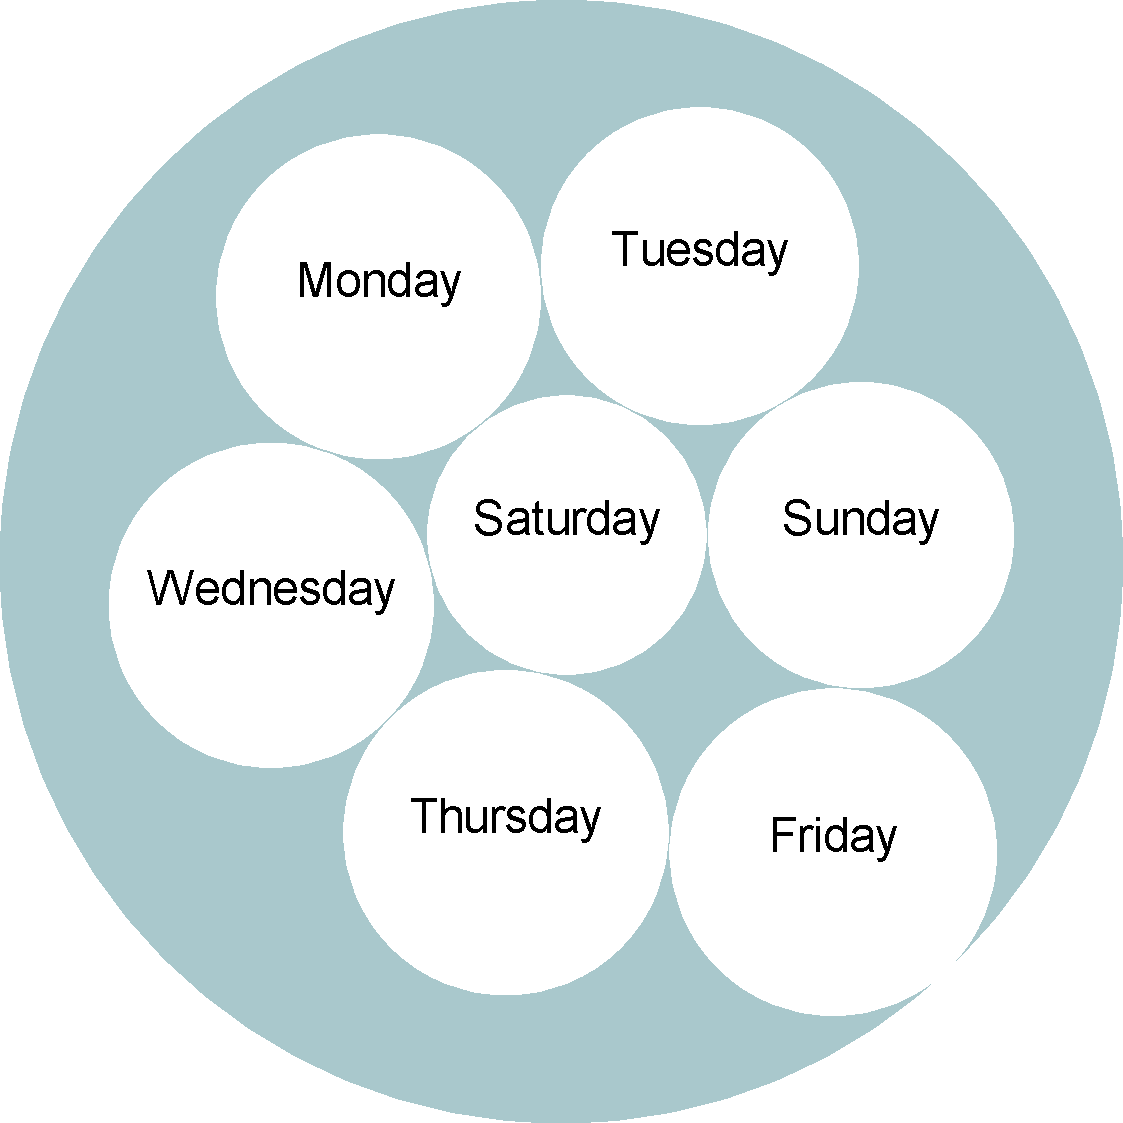
\includegraphics[width=0.45\textheight]{images/clusters_days.pdf}
	\hspace*{1.3em}%
	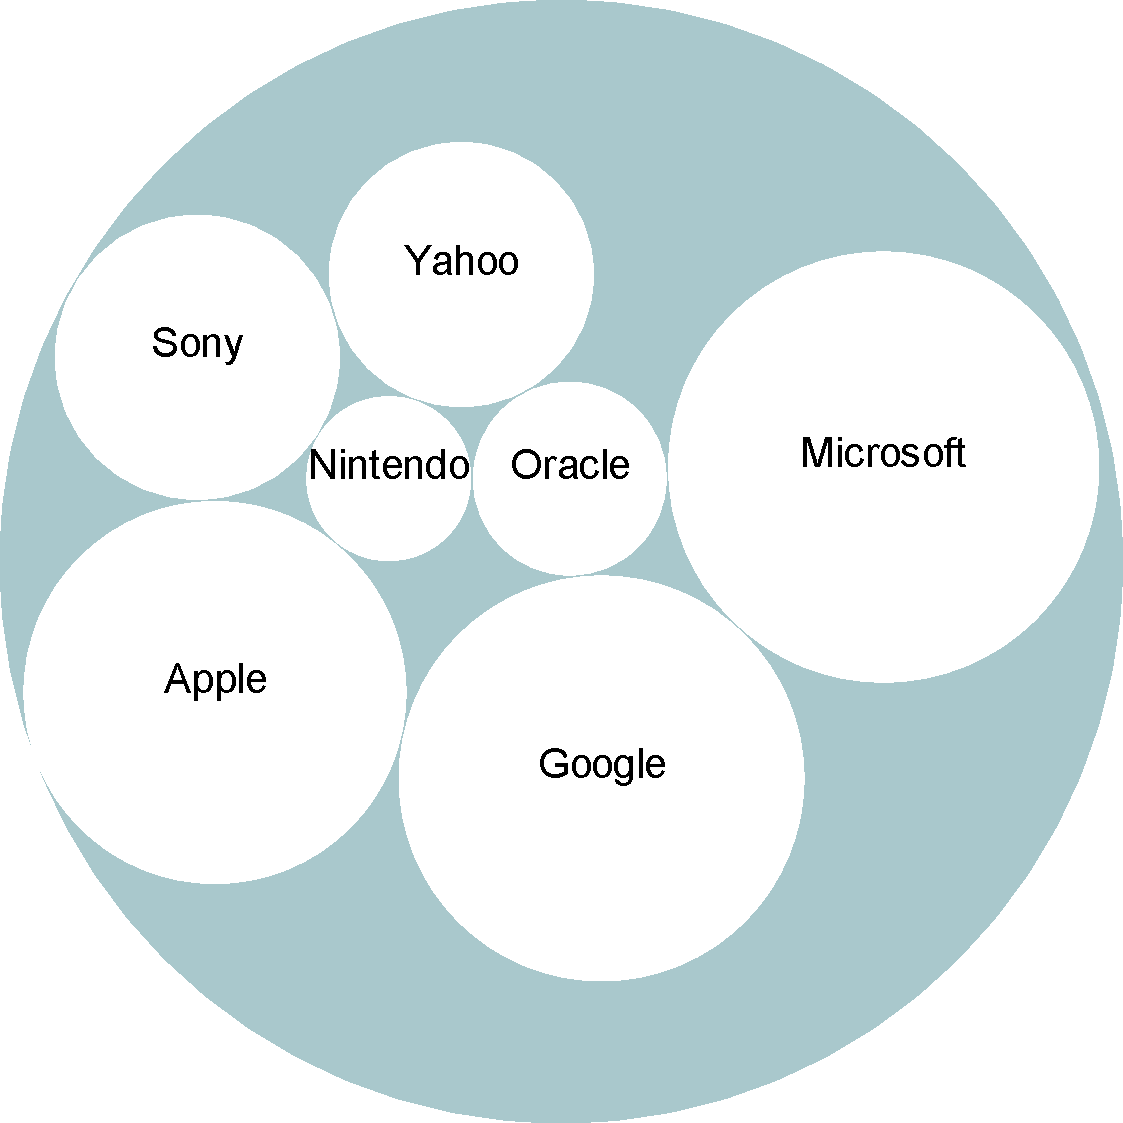
\includegraphics[width=0.45\textheight]{images/clusters_tech_companies.pdf}%
\end{center}
\pause

	\item Hand-crafted equivalence classes are called \textbf{part-of-speech tags}, and automatically induced equivalence classes are usually called \textbf{word classes} or \textbf{word clusters}
\end{itemize}
\end{frame}

% parts of speech
\begin{frame}{Parts of Speech and Word Clusters}
\begin{itemize}
	\item Part-of-speech example: \\[0.7em]
		\begin{scriptsize}
		\begin{tabular}{lllllllllll}
			Pierre & Vinken & , & 61 & years & old & , & will & join & the & board \\
			NNP & NNP & , & CD & NNS & JJ & , & MD & VB & DT & NN \\
		\end{tabular}
	\end{scriptsize} \\[1.0em]

	\item Word cluster example: \\[0.7em]
		\begin{scriptsize}
		\begin{tabular}{lllllllllll}
			Pierre & Vinken & , & 61 & years & old & , & will & join & the & board \\
			344 & 0 & 283 & 94 & 348 & 274 & 283 & 367 & 360 & 71 & 390 \\[0.8em]
		\end{tabular}
		\end{scriptsize}
	\pause
	\hspace*{-1.5em}\textbf{Differences}:
	\item Parts of speech have human-readable labels (eg.\ NN, VB), while word clusters usually just have numbers
	\item A word can have more than one part of speech (which depends on the context), while a word usually has just one word class
\end{itemize}
\end{frame}

\begin{frame}{Supervised, Unsupervised, Semi-supervised Learning}
\begin{itemize}
	\item \small{\textbf{Supervised learning} uses \textbf{manually-annotated data}} \hfill
		\raisebox{-2.0em}{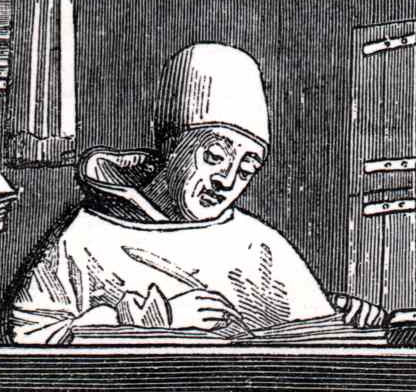
\includegraphics[width=0.13\textwidth]{images/scriptorium-monk-at-work-crop.jpg}}
	\begin{itemize}
		\pause
		\item It's usually evaluated on \textbf{accuracy} (or related idea) of `correct' label, given unannotated test input
		\pause
		\item The data's\textsuperscript{\scalebox{0.50}{$^1$}} usually expensive and small
	\end{itemize}
	\pause
	\item \textbf{Unsupervised learning} uses \textbf{unannotated data} \hfill
		\raisebox{-2.0em}{
\includegraphics[width=0.17\textwidth]{images/Bart-simpson-01.png}}
	\begin{itemize}
		\pause
		\item It's usually evaluated on the probability of the unannotated test input ($\propto$ \textbf{perplexity}), or a downstream task
		\pause
		\item The data's usually big and noisy. Just like the world around us.
	\end{itemize}
	\pause
	\item \textbf{Semi-supervised learning} uses \textbf{both} unannotated and annotated data
	\begin{itemize}
		\item It's usually evaluated just like supervised learning tasks
	\end{itemize}
\end{itemize}
\teeny{That's right: ``data is''\,.}
\end{frame}

\begin{frame}{Words \textit{vs}.\ Word Classes}
\begin{itemize}
	\item Using word classes reduces the number of parameters in language models, which means \textbf{generalization}
	\pause
	\item But, some sequences of words are \textbf{lexicalized}, meaning they are based on the specific words involved
	\pause
	\item For example:   ``\,It's raining cats and \underline{\hspace{2em}}\,''
	\pause
	\item Using word-based language models, the next word will probably be `\textit{dogs}'
	\pause
	\item But class-based LMs only see something like ``\,PRP VBZ VBG NNS CC \underline{\hspace{2em}}\,''
	\item So they would predict something like `\textit{shares}', if they were trained on the WSJ corpus
\end{itemize}
\end{frame}

\begin{frame}{How Many Word Classes Should I Use?}
	\begin{large}
	The more word classes you use, the closer you get to a word-based model \\[1.0em]

	\pause
	If you use a class-based LM by itself, more word classes is usually better, especially if you have a lot of training data \\[1.0em]

	\pause
	However if you interpolate a class-based LM with a word-based LM, fewer word classes is usually better, because you get complementary information
	\end{large}
\end{frame}

\begin{frame}{How Can You Cluster Words?}
\begin{itemize}
	\item If you represent words as vectors of real numbers, you can use general clustering algorithms like $k$-means clustering or agglomerative clustering
	\pause
	\item You can also use discrete versions of these two algorithms, to cluster words directly from plaintext
	\pause
	\item Discrete agglomerative word clustering is usually called \textbf{Brown clustering}
	\item Discrete $k$-means word clustering is usually called \textbf{exchange algorithm clustering}
\end{itemize}
\end{frame}

\begin{frame}{}
	\hspace*{-19.0em}%
	\scalebox{0.77}{%
		\usetikzlibrary{mindmap}
%\usetikzlibrary{positioning,shadows,shapes.geometric}
\providecommand{\mkcls}{\index{mkcls}\texttt{mkcls}}
    \begin{tikzpicture}
      \path[mindmap,
%every node/.style={concept,execute at begin node=\hskip0pt},
grow cyclic,
clockwise from=0,
level 1/.append style={level distance=12.2em, sibling angle=75},
level 2/.append style={level distance=7.5em,sibling angle=45},
level 3/.append style={level distance=5.5em,sibling angle=45},
clockwise from=-60,
%concept color=black,
text=white,
font=\Large
]
        node[concept] {Discrete \\ Word \\ Clustering}
        [clockwise from=-54]
        child[concept color=blue!50!black] {
            node[concept] {Exchange}
            [clockwise from=0]
            child { node[concept] {Orthotactics \\ \hrulefill \\ Clark} } % 2003
			child[concept color=green!20!blue] {
                node[concept] {Partially Lexicalized}
                child { node[concept] {Predictive \\ \hrulefill \\ Phrasal}
                    %child { node[concept] {BiDi \\ \hrulefull \\ ClusterCat} }
                }   
                child { node[concept] {Emami \& Jelinek} }
                child { node[concept] {Whittaker \& Woodland} } % 2001
            }
            child { node[concept] {Trigram \\ \hrulefill \\ MarLiN} } % 1998
            child { node[concept] {Bilingual} } % 1998
            child { node[concept] {{\tiny Metaheuristics} \\ \hrulefill \\ \mkcls{}} } % 1995
        }   
        child[concept color=brown] {
            node[concept] {Brown}
			[clockwise from=-67]
            child { node[concept] {Spectral \\ \hrulefill \\ Greedo} }
            child { node[concept] {Liang \\ \hrulefill \\ \texttt{brown-\\cluster}} }
        };  
    \end{tikzpicture}

	}%scalebox
\end{frame}


\begin{frame}{Brown Clustering (hierarchical clusters)}
\begin{enumerate}
	\item Assign the most frequent words to their own class
	\pause
	\item For the remaining words, assign the next most frequent word to the class giving the best likelihood of the training data
	\pause
	\item There is no step 3.
	\pause
	\item Optionally recursively merge the remaining classes, again based on likelihood
\end{enumerate}
\pause
\begin{itemize}
	\item Above is \href{http://people.csail.mit.edu/pliang/papers/meng-thesis.pdf}{Percy-style} Brown clustering, which can be more efficient than the original algorithm
	\pause
	\item The time complexity is $\mathcal{O}( |V| \times |C|^2 )$
	\item $|V|$ is the size of the vocabulary \\
	      $|C|$ is the number of word classes \\
	\pause
	\item Thus it's fairly fast for small clusters ($<400$), but slow for large clusters ($>800$)
\end{itemize}
\end{frame}

\begin{frame}{Exchange Algorithm (flat clusters)}
\begin{enumerate}
	\item Randomly assign each word to a class
	\pause
	\item For each word, change its word class to the one giving the best likelihood of the training data
	\pause
	\item Do the last step for a few times (maybe 10--20 iterations)
\end{enumerate}
\pause
\begin{itemize}
	\item Thus the basic time complexity is $\mathcal{O}(|V| \times |C| \times i)$
	\item $|V|$ is the size of the vocabulary \\
	      $|C|$ is the number of word classes \\
	      $i$ is the number of iterations
\pause
	\item There's a little more added complexity is how you calculate training-set likelihood
\end{itemize}
\end{frame}

\begin{frame}{Class-based Language Models}
\begin{itemize}
	\item So how do we use word classes as a language model?
	\pause
	\item The most common form ($c_i$ is the word class of word $w_i$):
	\begin{equation*}
		P(w_i|w_{i-1}) \,\triangleq\,  P(w_i | c_i) \, P(c_i | c_{i-1})
	\end{equation*}
	\vspace*{0.0em}

\scalebox{0.74}{%
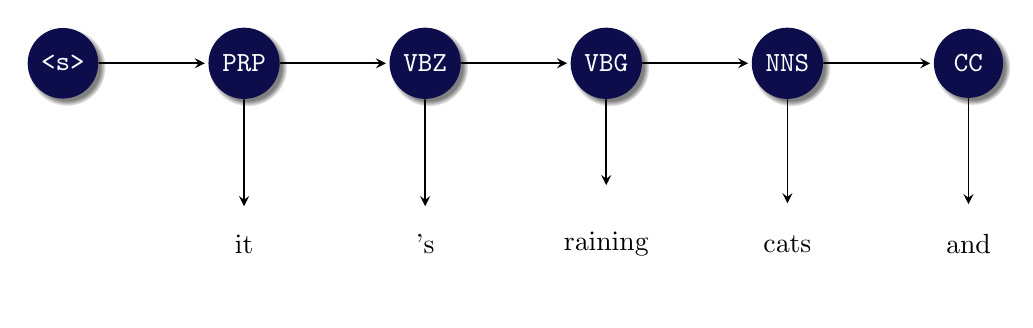
\begin{tikzpicture}[->,>=stealth,line cap=round,shorten >=1pt,auto,node distance=2.3cm,
                    semithick, initial text={},
					every state/.style={fill=darkblue,draw=none,text=white,circular drop shadow},
					accepting/.style={fill=white,draw=none,text=black,general shadow={fill=white, shadow scale=2}},
					hidden/.style ={white!95!black,text=black},
				]

  \node[state]				(s)				   {\texttt{<s>}};
  \node[state]				(C1) [right of=s]  {\texttt{PRP}};
  \node[state,accepting]	(w1) [below of=C1] {it};
  \node[state]				(C2) [right of=C1] {\texttt{VBZ}};
  \node[state,accepting]	(w2) [below of=C2] {'s};
  \node[state]				(C3) [right of=C2] {\texttt{VBG}};
  \node[state,accepting]	(w3) [below of=C3] {raining};
  \node[state]				(C4) [right of=C3] {\texttt{NNS}};
  \node[state,accepting]	(w4) [below of=C4] {cats};
  \node[state]				(C5) [right of=C4] {\texttt{CC}};
  \node[state,accepting]	(w5) [below of=C5] {and};

  \path (s)  edge              node {} (C1)
        (C1) edge              node {} (C2)
             edge              node {} (w1)
        (C2) edge              node {} (C3)
             edge              node {} (w2)
        (C3) edge              node {} (C4)
             edge              node {} (w3)
        (C4) edge              node {} (C5)
             edge              node {} (w4)
        (C5) edge              node {} (w5)
		 ;
\end{tikzpicture}
}

\pause
\item Notice $c_i$, which is called a \textbf{bottleneck variable}
\item The history is `squeezed' through this point, in order to summarize and generalize the history
\end{itemize}
\end{frame}


\begin{frame}{Predictive Exchange and Conditional Exchange}
\begin{itemize}
	\item The previous model is used in both Brown clustering and exchange algorithm clustering to determine the likelihood of the training set.
	We can use different models as well.
	\pause
	\item The \emph{predictive exchange algorithm} uses this model:
	\begin{equation*}
		P(w_i|w_{i-1}) \,\triangleq\, P(w_i | c_i) \, P(c_i | w_{i-1})
	\end{equation*}
	\item The \emph{conditional exchange algorithm} uses this model:
	\begin{equation*}
		P(w_i|w_{i-1}) \,\triangleq\, P(w_i | c_{i-1})
	\end{equation*}
\end{itemize}
\end{frame}



\begin{frame}{Uses of Word Clusters}
\begin{footnotesize}
\begin{block}{Machine Translation}
	\begin{itemize}
		\itemsep-0.4em
		\item Word alignment {\tiny (Brown et al, 1993; Och \& Ney, 2000)} \nocite{brown-etal1993,och-ney2000}
	\item {\footnotesize Factored/class-based translation models} \nocite{koehn-hoang2007,wuebker-etal2013,mediani-etal2012} {\tiny (Koehn \& Hoang, 2007; {\it inter alia})} %Wuebker et al, 2013; Mediani et al, 2012)}
		\item Reordering models {\tiny (Cherry, 2013)} \nocite{cherry2013}
		\item Preordering {\tiny (Stymne, 2012)} \nocite{stymne2012}
		\item Target-side inflection {\tiny (Chahuneau et al, 2013)} \nocite{chahuneau-etal2013}
		\item Syntax-augmented machine translation {\tiny (Zollmann \& Vogel, 2011)} \nocite{zollmann-vogel2011}
		\item Sparse word features {\tiny (Haddow et al, 2015)} \nocite{haddow-etal2015}
		\item Operation sequence models {\tiny (Durrani et al, 2014)} \nocite{durrani-etal2014}
		%\item {\tiny ()} \nocite{}
	\end{itemize}
\end{block}
\pause
\begin{block}{Other NLP Tasks}
	\begin{itemize}
		\itemsep-0.4em
		\item Training Neural Net Lang.\ Models {\tiny (Goodman, 2001; Mnih \& Hinton, 2009; ...)} \nocite{goodman2001a,mnih-hinton2009}
		\item Parsing {\tiny (Koo et al, 2008; Candito \& Seddah, 2010; Kong et al, 2014)} \nocite{koo-etal2008,candito-seddah2010,kong-etal2014}
		\item Semantic Parsing {\tiny (Zhao et al, 2009)} \nocite{zhao-etal2009}
		\item Chunking {\tiny (Turian et al, 2010)} \nocite{turian-etal2010}
		\item NER {\tiny (Miller et al, 2004, {\it inter alia})} \nocite{miller-etal2004,liang2005,ratinov-roth2009,turian-etal2010,ritter-etal2011}
		\item Tagging of Twitter Feeds {\tiny (Owoputi et al, 2013; Nooralahzadeh et al, 2014)} \nocite{owoputi-etal2013,nooralahzadeh-etal2014}
		\item Structure Transfer {\tiny (T\"{a}ckstr\"{o}m et al, 2012)} \nocite{tackstrom-etal2012}
		\item Discourse Relation Discovery {\tiny (Rutherford \& Xue, 2014)} \nocite{rutherford-xue2014}
	\end{itemize}
\end{block}
\end{footnotesize}
\end{frame}


\begin{frame}[allowframebreaks]
 \frametitle{References}
 \begin{tiny}
 \begin{spacing}{0.70}
\bibliographystyle{apalike}
\bibliography{bib}
\addcontentsline{toc}{section}{References}
 \end{spacing}
 \end{tiny}
\end{frame}



% \begin{frame}{}
% \begin{block}{}
% \begin{itemize}
% 	\item 
% 	\item 
% 	\item 
% \end{itemize}
% \end{block}
% \end{frame}


\end{document}
